\chapter{Reactive Component Model \label{model}}

In this chapter, we present a model for composing and decomposing reactive programs via \emph{reactive components}.
The model is biased toward practical software development even as it enforces properties based in formal methods.
Consequently, the model favors utility, practicality, flexibility, and ease of implementation.

%% \paragraph{Formal models and software engineering.}
%% I claim that most of the software that is ``put into production'' will never be proved formally correct.
%% This is a function of economics since modeling and constructing proofs is a labor-intensive process that can only be justified for safety or mission critical software.
%% However, I would argue that the development and application of formal models are critical to software engineering.
%% To illustrate, consider \emph{structured programming}~\cite{dahl1972structured}.
%% Structured programming assumes an abstract machine that executes programs that are restricted to a small set of well-defined control structures and assignment statements.
%% A program written in this form can be reasoned about directly from the text by formulating a Hoare-triple for each statement.
%% Structured programming opened the door for \emph{structured programming languages} which are also based on well-defined control structures and evaluation semantics.
%% Thus, while very few programmers will prove their structured programs correct, all of them informally use structured programming when they are fixing a bug revealed by a unit test or analyzing a core dump in a debugger.
%% Structured programming languages reduced the accidental complexity associated with writing the same program in assembly language.

%% The realm of reactive programs is waiting for a similar reduction in accidental complexity.
%% Taking a hint from structured programming, I believe two things are required.
%% First, we must write reactive programs against an easy-to-reason-about abstract machine instead of low-level interfaces like atomic instructions and thread libraries.
%% Second, we must restrict the form of reactive programs so that they can be reasoned about from the text.
%% I hope the proposed model of reactive systems is a step toward toward this goal.

\section{Features of the Model}

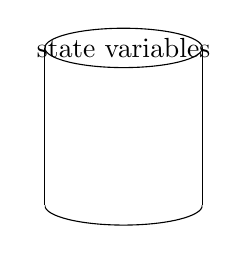
\begin{tikzpicture}
\node (sv) at (0,0) {state variables};
\begin{scope}
\clip (-1,-2.25) rectangle (1, -2);
\draw (0,-2) ellipse (1 and .25);
\end{scope}

\draw (0,0) ellipse (1 and .25);
\draw (-1,0) -- (-1,-2);
\draw (1,0) -- (1,-2);
\end{tikzpicture}

\begin{figure}[H]
\centering
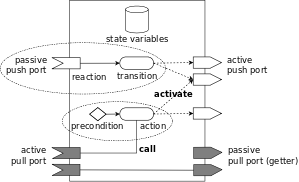
\includegraphics{reactive_component.png}
\caption{Diagram depicting the features of a reactive component\label{reactive_component}}
\end{figure}

Figure~\ref{reactive_component} shows the major features of a reactive component.
As in other state-based formal models like UNITY~\cite{chandy1989parallel} and I/O Automata~\cite{nancy1996distributed}, the core of a reactive component in this model is a set of \emph{state variables} and a set of atomic \emph{transitions} that manipulate those state variables.
When reasoning about a system, behavior is expressed as propositions over the state variables where the propositions are derived from the transitions.
The contribution that this work makes to existing state-based formal models of reactive systems is a combination of interface elements and composition semantics that allow reactive programs to be composed in a principled way.

For example, an \emph{active push port} allows a transition in one component to be linked to a transition in another component such that the resulting combined transaction is atomic.
Active push ports allow reactive components to publicize their behavior.
An active push port may be \emph{bound} to and conditionally \emph{activate} zero or more \emph{passive push ports}.
A passive push port names the corresponding transition that will be executed when the passive push port is activated.
This combination of passive push port and transition is called a \emph{reaction} because it reacts to a transition in another component.

The atomic linkage of a transition in one component to a transition in another component through the push port mechanism allows the properties of each component to be related to one another and complex systems to be constructed by composing simpler systems.
Transitions that are not executed via a passive push port have a precondition that nominates them for execution by a weakly fair scheduler.
The combination of a precondition and transition is called an \emph{action} because it is a voluntary transition under the control the containing component.

An \emph{active pull port} represents an immutable external data dependency.
The component may \emph{call} an active pull port to yield a value required in a transition.
Active pull ports must be bound to a \emph{passive pull port} which resembles a function returning a value, e.g., a getter or a predicate.
Where push ports allow components to publicize their behavior, pull ports allow components to safely publicize their internal state for use by other components.

Composition in the reactive component model has two main features.
The first is recursive encapsulation where a state variable in one component may represent an instance of another reactive component.
The second is the ability to bind push ports and pull ports through an \emph{explicit} set of \emph{bindings}.
The decision to use an explicit set of bindings as opposed to implicit named-based matching is more in keeping with the goals and techniques of practical software development since it facilitates the use of software developed under different naming conventions, i.e., third-party software.
A third minor feature called \emph{exporting} is the ability of an encapsulating component to adopt interface elements of its sub-components without defining complimentary ports and transitions that do nothing but forward an activation or call.
The ability to publicize behavior and state and the ability to assemble well-defined behavior from existing behaviors in a straight-forward and flexible way are the defining characteristics of the reactive component model.

\begin{figure}
\centering
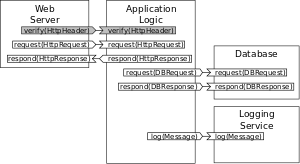
\includegraphics{web_server.png}
\caption{Diagram of a web application built using reactive components\label{web_server}}
\end{figure}

To illustrate the utility of component interfaces and composition, we now present a design for a web application or web server using reactive components in figure~\ref{web_server}.
The web application consists of five reactive components.
The first is an unnamed top-level component representing the complete application.
This component has four sub-components representing a web server, the application logic, a database, and a logging service.
The ports of the application logic component have been bound to the corresponding ports in the web server, database, and logging service components.
The interface of a component, which consists of its ports, provides insight into the behavior of a component.
For example, based on the interface of the web server component we may expect it to 1) verify incoming HTTP requests\footnote{A production web server may verify that the requested HTTP method can be applied to the given URI, that content length limits are respected, that content types are supported, etc.}, 2) pass on valid HTTP requests to the application, and 3) send HTTP responses to the web client.

Figure~\ref{web_server} also demonstrates how reactive programs can be constructed by composing reactive components, so that a developer may focus on the application logic and use already developed components for the web server, database, and logging service.
Furthermore, one can imagine developing three stateless components surrounding the application logic that do nothing but translate messages to and from application specific message types to the generic types required by the web server, database, and logging service.
The application logic, then, is completely isolated from the surrounding libraries and may be tested by providing mock components for the web server, database, and logging service.
The application logic itself has a well-defined interface and could be reused, say, by implementing a graphical front-end to drive the application instead of a web service.

\paragraph{State variables.}
A key part of the internal core of a reactive component is a set of state variables.
When modeling, the state variables are the subject of the various propositions that demonstrate the behavior of the system.
When implementing, the state variables are manipulated by the various assignment statements that constitute the transitions.
As in other formal models, the types of the state variables may be selected to make writing proofs easier.
That is, the types of state variables are mathematically friendly like integers, sets, and lists.
Implementations of the reactive component model must provide a type system that allows the state variables to be realized on a given machine.
The type of a state variable may be a reactive component type which facilitates recursive encapsulation.
For modeling purposes, state variables typically have \emph{value semantics} meaning we need not reason about references.
As a practical concession, however, we will introduce pointers for building arbitrary linked data structures since we advocate an imperative state-based implementation and describe the issues of introducing pointers into the reactive component model.

\paragraph{Atomic state transitions.}
The rest of the internal core of a reactive component is a set of atomic state transitions that manipulate the state variables.
A precise definition of the atomicity of state transitions will be deferred to the discussion on composition and execution.
State variables and state transitions are private, meaning that transitions can only refer to the state variables of the associated reactive component and a transition in one reactive component can only be linked to a transition in another component through the composition mechanisms.
Thus, all initialization and updates to state variables can be determined by examining the transitions of the corresponding component.
Thus, composition is \emph{compositional}, meaning that a property established for a reactive component independent of context can never be violated since the set of transitions from which the properties were derived is fixed.
State transitions must be deterministic meaning that the next value of every state variable is uniquely and well defined.

The reactive component model does not prescribe a specific language for encoding state transitions.
The language used depends on the goals and tastes of the one developing or analyzing the model.
For example, expressing transitions using the programming language of UNITY~\cite{chandy1989parallel} may allow the modeler to extract proofs from the text, a major goal of UNITY.
The approach used by I/O Automata~\cite{nancy1996distributed} is to specify the condition established by each transition.
The approach used by the implementation presented in this dissertation uses a C-like language augmented for port activations to encode the state transitions.
%% from Dr. Gill
%% which aims to allow models to be incorporated directly into standard software environments.
%% This isn't accurate.  Compatibility with existing software is not the goal nor should it be a goal as existing software is based on threads which cannot reasonably be integrated with reactive components.

\paragraph{Actions, reactions, push ports, and composition.}
A state transition is either part of an action or reaction.
An \emph{action} is a state transition whose execution is under the control of the component to which it belongs.
The action is guarded by a \emph{precondition} that is guaranteed to be true when the action is executed.
The precondition is a Boolean expression that determines if the action is \emph{enabled} or \emph{disabled}.
If the precondition is absent, it is assumed to be true.

A \emph{reaction} is a state transition whose execution is under the control of another action or reaction.
Thus, we require a mechanism for linking a reaction to an action or another reaction.
To do this, we introduce the notion of a \emph{push port}.
A push port is a typed interaction point consisting of an active side that conditionally \emph{activates} the port and provides arguments to the port, and a passive side that \emph{reacts} to the port and may access the arguments provided by the active side.
The transition associated with a passive push port is executed atomically with the transition that activates the active push port.

\paragraph{Execution.}
As with UNITY~\cite{chandy1989parallel} and I/O Automata~\cite{nancy1996distributed}, we assume the existence of a weakly fair scheduler that \emph{selects} and \emph{executes} enabled instance/action pairs.
Selection is \emph{serial}, meaning that one action is considered (and therefore executed) at a time.
Thus, each action is atomic with respect to all other actions.
Selection is also \emph{non-deterministic}, meaning that the scheduler is free to select any instance/action pair according to weak fairness (which is described below).
This falls in line with the common practice of modeling concurrency with non-deterministically scheduled atomic actions as is done in UNITY~\cite{chandy1989parallel}, I/O Automata~\cite{nancy1996distributed}, and the Actor Model~\cite{agha1985actors}.

A \emph{trace} is the sequence of instance/action pairs executed by the scheduler.
Weak fairness says that all instance/action pairs are selected an infinite number of times in an infinite run of the system.
Finite runs, indicated by a finite trace, occur when a system reaches \emph{fixed-point}, a state where all preconditions are false.
In this state, further selection is unnecessary.

The key point to understanding weak fairness is the difference between selections and execution.
To illustrate, consider a component consisting of a single Boolean flag $b$ that is initially false and three actions labeled $A$, $B_0$, and $B_1$.
Action $A$ is enabled when $b = false$ and sets $b$ to true.
Actions $B_0$ and $B_1$ are enabled when $b = true$ and set $b$ to false.
A trace for this component resembles $ABAB \ldots$ where $B$ represents either $B_0$ or $B_1$.
Thus, an infinite trace will contain an infinite number of $A$s.
However, the same trace may contain an infinite number of $B_0$s with no $B_1$s, an infinite number of $B_1$s with no $B_0$s, or some combination of $B_0$s and $B_1$s.
These extreme cases illustrate weak fairness.
Assume the trace contains no $B_1$s.
From this, we can conclude that the scheduler always selected $B_0$ when $b = false$, which occurred an infinite number of times.

When an action is executed it may conditionally activate various push ports.
If these ports are bound to reactions, the reactions will be executed, their push ports conditionally activated and so on.
We divide a state transition into two steps called the \emph{immutable step} and the \emph{mutable step}.
Logically, a transition assigns values to a set of state variables.
This can be modeled as a multiple assignment statement with a left-hand side (LHS) consisting of a list of state variables and a right-hand side (RHS) consisting of a list of expressions that provide the next value for the corresponding state variable.
The immutable step corresponds to the computation of the RHS in a state transition.
The mutable step corresponds to the update of the values on the LHS with the values on the RHS.
When transitions are linked with composition, we must relate the mutable and immutable step in a state transition to the mutable and immutable steps in all dependent state transitions.
Let $A$ be a transition and $B$ be a transition that depends on $A$.
Let $A_I$ be the immutable step of $A$, $A_M$ be the mutable step of $A$, $B_I$ be the immutable step of $B$, and $B_M$ be the mutable step of $B$.
For the sake of argument, assume that $A_I$ reads variables that are written in $B_M$ and that $B_I$ reads variables that are written in $A_M$.
We require that $A_I$ be evaluated before $A_M$, $B_I$ be evaluated before $B_M$, and $A_I$ be evaluated before $B_I$ since activation is conditional.
This leaves three possible sequences of steps:
\begin{itemize}
\item $A_I A_M B_I B_M$.  In this sequence, a variable is first updated in $A_M$ and then the updated value is read in $B_I$.  The issue with this interpretation is that it does not compose well.  Ideally, we would like to be able to rewrite the transition as a single transition consisting of a single immutable step and mutable step.
\item $A_I B_I A_M B_M$ and $A_I B_I B_M A_M$.  These sequences resolve the issue with the first sequence by providing a clear immutable step and mutable step.
\end{itemize}
Thus, with respect to composed state transitions, all immutable steps (which includes all push port activations) are performed before all mutable steps.

\section{Illustrative Example}
To illustrate the behavior of reactive components under this model, we rewrite the \emph{Clock automaton} example in \cite{nancy1996distributed} using reactive components.
The Clock automaton consists of a free-running counter and flag used to implement a request-response protocol.
Our Clock automaton is defined in figure~\ref{clock_component}.
The state variables are identified with \verb+var+ and their initial values are provided.
The component contains a reaction named \verb+request+ for receiving requests to sample the current value of the counter.
The component also contains an active push port named \verb+clock+ for communicating the sampled value of the counter.
The first action, \verb+Tick+, is an action that increments the free-running counter.
The absence of a precondition means this action is always enabled.
The second action, \verb+Clock+, is conditioned on the flag variable (which indicates that a request has been made) which when it executes resets the flag and communicates the value of \verb+counter+ by activating the \verb+clock+ port.
A simple client (for the Clock component) that perpetually samples the clock is shown in figure~\ref{client_component}.

\begin{figure}
\begin{verbatim}
component Clock {
  var int counter (0)
  var bool flag (false)
  push clock(int t)

  Tick: counter := counter + 1

  reaction request() flag := true

  Clock: flag -> flag := false activates clock(counter)
}
\end{verbatim}
\caption{Definition of the Clock component\label{clock_component}}
\end{figure}

\begin{figure}
\begin{verbatim}
component Client {
  var bool flag (false)
  push request()

  Request: !flag -> flag := true activates request()

  reaction clock(int t) flag := false || /* do something with t */
}
\end{verbatim}
\caption{Definition of a client of the Clock component\label{client_component}}
\end{figure}

In isolation, the Clock component will increment its counter forever and the client component will make a request and then stop.
In order to make the two components work together, we must compose them.
Figure~\ref{system_component} shows a system component that instantiates a Clock component and a client component and binds the corresponding push ports in each instance.
In this system, the client's \verb+Request+ action will be executed activating the \verb+request+ port which in turn causes the \verb+request+ reaction in the Clock to be executed.
Eventually, the Clock's \verb+Response+ action will be executed activating the \verb+clock+ port which in turn causes the \verb+clock+ reaction in the client to be executed with the current value of the Clock's counter.
In between these actions, the \verb+Tick+ action of the Clock is incrementing the counter.

\begin{figure}
\begin{verbatim}
component System {
  var Clock clock
  var Client client

  bind {
    client.request -> clock.request
    clock.clock -> client.clock
  }
}
\end{verbatim}
\caption{Definition of a system component\label{system_component}}
\end{figure}

\section{Properties of Composition}
In this section, we examine various features related to reactive components and composition.
Substitutional equivalence for reactive components is demonstrated by outlining a procedure for in-lining sub-components.
Hazards of composition, namely, non-deterministic state transitions resulting from conflicting and recursive composition, are identified and a means of detecting is proposed.
The issue of decomposition is considered and \emph{pull ports} are introduced as a mechanism for decomposition.
Finally, the points of principled composition presented in chapter~\ref{introduction} are evaluated against reactive components.

\paragraph{Substitutional equivalence.}
Substitutional equivalence means that an instance of a component can be replaced with its definition and the result is a well-defined entity in the model.
To this end, a procedure for substituting the definition of a component for an instance involves:
\begin{enumerate}
\item Renaming and adding all state variables, ports, actions, and reactions to the parent component.
\item Simplifying bindings and ports by substituting the transitions associated with reactions into the action or reaction that activates the port in question.
\end{enumerate}
To illustrate, figure~\ref{se1} shows the result of substituting state variables, ports, actions, and reactions into the system component.
Figure~\ref{se2} shows the second step of simplifying bindings, ports, and state transitions.
The result is a reactive component whose ``size'' in terms of state variables, actions, and reactions is the sum of the sizes  of its constituent components.
Substituting the member instances in the system component confirms the intuition that the client flag variable and clock flag variable are the same since 1) initially they have the same value and 2) they take on the same value in every state transition.

\begin{figure}
\begin{verbatim}
component System {
  /* Substitution of clock component. */
  var int clock_counter (0)
  var bool clock_flag (false)
  push clock_clock(int t)

  clock_Tick: clock_counter := clock_counter + 1

  reaction clock_request() clock_flag := true

  clock_Clock: clock_flag -> clock_flag := false activates clock_clock(clock_counter)

  /* Substitution of client component. */
  var bool client_flag (false)
  push client_request()

  client_Request: !client_flag -> client_flag := true activates client_request()

  reaction client_clock(int t) client_flag := false || /* do something with t */

  bind {
    client_request -> clock_request
    clock_clock -> client_clock
  }
}
\end{verbatim}
\caption{Substitution of state variables, ports, actions, and reactions into system component\label{se1}}
\end{figure}

\begin{figure}
\begin{verbatim}
component System {
  var int clock_counter (0)
  var bool clock_flag (false)
  var bool client_flag (false)

  clock_Tick: clock_counter := clock_counter + 1

  clock_Clock: clock_flag -> clock_flag, client_flag := false, false ||
    /* do something with clock_counter */

  client_Request: !client_flag -> client_flag, clock_flag := true, true
}
\end{verbatim}
\caption{Simplification of ports, bindings, and transitions in expanded system component\label{se2}}
\end{figure}

\paragraph{Determinism and composition.}
The result of composing two well-defined reactive components may yield a system that is non-deterministic.
The two ``hazards'' that must be avoided are non-deterministic assignment to state variables and recursively activated reactions.
To illustrate these hazards, we model an individual transaction as a directed graph $G = (N,V)$ where each node $N=(i,t)$ is an instance/transition pair and the edges are modeled as function $V: N \to N$ that encodes the causal relationships induced by port activations and bindings.
A transaction graph has a distinguished root $r \in N$ where the transition corresponds to an action while all of the other nodes in the graph correspond to reactions.

Non-deterministic assignment results when the next value for a state variable is not well defined due to the inclusion of two or more transitions that operate on the state variable.
To illustrate, consider a component $A$ that contains two passive push ports.
One of the passive push port is linked to a transition that sets a flag to false while the other passive push port is linked to a transition that sets the same flag to true.
Suppose that the two push ports of $A$ are activated by the same action.
This may happen directly, i.e., the action activates a push port that is bound to both push ports in $A$, or indirectly, i.e., an arbitrary but bounded number of reactions and port activations are placed between the action and ports of $A$ through composition.
The resulting system is non-deterministic because the value of the flag after the action may either be true or false.
If the underlying transformational language admits pointers, then the problem of determining if two transitions operate on the same state variable is undecidable in general.
A necessary (but not sufficient) condition for non-deterministic assignment from composition is summarized by the following predicate $NDA(G): \exists (i_1, t_1), (i_2, t_2) \in G.N, i_1 = i_2, t_1 \ne t_2$ which says that the graph must have two different transitions involving the same instance.

A recursively activated transition occurs when the transaction graph has a cycle.
The execution of such a transaction may result in well-defined next values for all state variables assuming that 1)~the recursion is bounded and 2)~the parameters passed to every reaction result in identical computations.
Both of these problems are undecidable in general.

The difficulty of detecting composition that results in non-deterministic assignments suggests that these problems are best checked by a machine.
That is, an implementation of reactive components may require that $NDA(G)$ be false for all transaction graphs in the system.
Similarly, an implementation may restrict composition to prevent the formation of cycles.
Both of these approaches are used by the implementation described in chapter~\ref{implementation}.

\paragraph{Decomposition, getters, and pull ports.}
Substitutional equivalence implies that the process may be reversed and that sub-components may be ``factored out'' of an existing component, e.g., for reuse with other components.
%% One motivation for extracting sub-components is to support the software engineering practice of refactoring where common code is extracted so that it can be reused in various places.

Another motivation is increased performance through parallelism.
Recall that true concurrency in reactive components is modeled as the non-deterministic selection and serial execution of actions.
Two actions can be safely executed concurrently if it can be shown that the state variables involved in each action are disjoint.
As previously mentioned, making this determination is undecidable in the general case.
However, the problem becomes decidable if the component instance is used as a proxy for its constituent state variables.
Let $RW: t \to \{ READ, WRITE \}$ be a function that maps a transition to value indicating that variables are read-only during the transition or written in some way.
Two instance/transition pairs are independent if either the instances are different or at most one of the transition writes the variables of the instance
\begin{displaymath}
I((i_1, t_1), (i_2, t_2)): i_1 \ne i_2 \lor \lnot (RW(t_1) = WRITE \land RW(t_2) = WRITE)
\end{displaymath}
Two transaction graphs are independent if all of their nodes are independent $IG(N_1, N_2) = \forall (i_1, t_1) \in N_1, (i_2, t_2) \in N_2 \; I((i_1, t_1), (i_2, t_2))$.
The significance of the preceding analysis is that the determination about what actions can be executed concurrently becomes machine checkable due to the strong guarantee that state variables belonging to an instance can only be modified in the transitions of that instance.

To illustrate the mechanisms required for decomposition, we will factor out a Counter component from the Clock component of figure~\ref{clock_component} and then rewrite the Clock component using the Counter component.
Upon inspection, the \verb+Tick+ action and \verb+request+ reaction can be executed concurrently since the state variables involved in each transition are disjoint.
The Counter component consists of the \verb+counter+ state variable.
The \verb+Tick+ action can be moved to the Counter component without complication.
The \verb+Clock+ action \emph{reads} the value of \verb+counter+ which suggests a mechanism for accessing the state variables in a component.
Thus, we introduce the notion of a \emph{getter} which can be called on a component to produce a value.
A getter is not allowed to modify the state of a component and may only be invoked in the immutable phase.
These semantics preserve the strict separation of immutable phase and mutable phase.
When analyzing composition, a getter is treated like a transition that reads the state variable of the corresponding instance.
The Counter component is shown in figure~\ref{counter_component} and figure~\ref{factored_clock_component} shows the corresponding Clock component.
The \verb+getCounter+ method returns the current value of the counter.

\begin{figure}
\begin{verbatim}
component Counter {
  var int counter (0)

  Tick: counter := counter + 1

  getCounter() int {
    return counter
  }
}
\end{verbatim}
\caption{Definition of the Counter component\label{counter_component}}
\end{figure}

\begin{figure}
\begin{verbatim}
component Clock {
  var Counter c
  var bool flag (false)
  push clock(int t)

  reaction request() flag := true

  Clock: flag -> flag := false activates clock(c.getCounter())
}
\end{verbatim}
\caption{Definition of the Clock component using the Counter component\label{factored_clock_component}}
\end{figure}

The logic associated with the \verb+flag+ state variable represents a generic request-response protocol except for the call to \verb+c.getCounter()+.
To indirect the call to \verb+c.getCounter()+ we introduce the notion of a \emph{pull port}.
A pull port represents an external value dependency.
A component can demand a value from the pull port in the immutable phase.
Like push ports, pull ports have an active and passive side.
The active side represents the caller and the passive side represents the callee.
Getters are sufficient to realize the passive side of a pull port.
Every active pull port must be bound to exactly one passive pull port via composition.
Figure~\ref{flag_component} shows a component representing the request/response protocol using a pull port \verb+getValue+.
Figure~\ref{factored2_clock_component} shows the Clock component written in terms of the Counter and Flag components.
An \verb+export+ directive allows ports in sub-components to be available in the interface of the encapsulating component.

\begin{figure}
\begin{verbatim}
component Flag {
  var bool flag (false)
  pull getValue() int
  push response(int t)

  reaction request() flag := true

  Response: flag -> flag := false activates response(getValue())
}
\end{verbatim}
\caption{Definition of the Flag component\label{flag_component}}
\end{figure}

\begin{figure}
\begin{verbatim}
component Clock {
  var Counter c
  var Flag f
  push request()
  push clock(int t)

  bind {
    c.getCounter -> f.getValue
  }

  export f.request as request
  export f.response as clock
}
\end{verbatim}
\caption{Definition of the Clock component using the Counter and Flag components\label{factored2_clock_component}}
\end{figure}

Pull ports have compositional hazard similar to the recursive activation hazard of push ports.
A cycle in the graph of composed pull ports is equivalent to a recursively defined function.
The recursion may be bounded but this is undecidable in the general case.
Consequently, an implementation may reject recursively defined push ports.

\paragraph{Principled composition.}
The goal of this section is to describe how reactive components satisfy principled composition.
\begin{enumerate}
\item The reactive component model defines a reactive component as the basic unit of composition.
A reactive component consists of a set of state variables and transitions.
The interface of a reactive component consists of push ports, and pull ports.
Composition is supported through recursive encapsulation and explicit port binding.

\item The result of composition is either well-defined due to the atomic nature of transactions or illegal due to non-determinism.

\item Reactive components support recursive encapsulation.

\item The external or visible behavior of a reactive component can be traced through its interface, specifically its push ports.
The internal details of a component can often be abstracted away to permit reasoning about the behavior of a composed system at various levels of detail.

\item Composition in reactive components is compositional since all updates to state variables are under the control of the transitions of the encapsulating reactive component.
Composition cannot ``undo'' a property established for a component.

\item Reactive components are subject to substitutional equivalence.
\end{enumerate}

\section{Summary}
In this chapter, we presented the reactive component model for reactive programs.
A reactive component consists of a set of state variables and transitions that are private to the component.
The interface of a reactive component consists of push ports, which allow a component to trigger a transition in another component, and pull ports, which allow a component to access the state of another component.

Composition is achieved through recursive encapsulation and explicit port binding.
Transitions that are linked through composition form an atomic transaction that allows the properties of one component to be related to another component.
Composition achieves the principles outline in chapter~\ref{introduction}.
The definitions of sub-components can be substituted into the containing component resulting in an equivalent system (substitutional equivalence).
Similarly, sub-components may be ``factored out'' by using pull ports and getters to safely access the state of the sub-components.
Non-deterministic state transitions resulting from composition can be detected by analyzing over component instances instead of individual state variables.
